\documentclass[../document]{subfiles}

\begin{document}

\section{Sprint 3}

\subsection{Introduction}
The following chapter includes all the documentation regarding the third sprint. This sprint will last 10 days and will take place from October 22 to October 31. The team will spend most of the time on integrating all the modules. Testing and improving current code.

\subsection{Sprint Planning}
Our main goals in this sprint has been focused on integration of modules, testing, and improving the visualiser. We plan on using a total of 124 hours for this sprint for implementation and 150 hours for documentation. We have a total of five work days planned for this sprint, which translates to 40 hours per person and with 7 group members it totals to 280 hours of possible work time during the sprint. Just like in the past sprints, we will most likely overestimate the time to work. We feel that it is better to overestimate than underestimate the time taken, as we are able to have a time buffer, in case we encounter any problems.

Most of the sprint workload will be split equally in between improving and documenting the visualiser, finishing the working prototype by integrating the database and sensors fully, and doing testing. Most of the tests in this sprint will be taken from the test plan document that can be found in \sectionfullref{test_plan}, and therefore some tests may be repeated from previous sprints. We will also use substantial time to work on documentation during this sprint.

\subsection{Sprint Goals}
The goal of this sprint is to make the visualiser look better, complete the prototype by integrating all the modules, and finish the system tests. Therefore we have three main goals this sprint:
\begin{enumerate}
	\item
	Improve the look of the visualiser.
	\item
	Finish integrating the system, from sensors to visualiser.
	\item
	Complete the tests as seen in our test plan.
\end{enumerate}

\subsection{Sprint Backlog}

Below is the sprint backlog in the form of a table, listing all the tasks we plan on working on in this sprint. We also include the estimated working hours for each task as well as the actual amount of work spent on each task, as we complete the tasks in the sprint. The tasks also include priority, which will help the group direct their focus on the most important sub-tasks first.

\begin{table}[H]
\caption{Sprint Backlog}
\centering
\begin{tabularx}{\textwidth}{|l|X|l|L{1.7cm}|L{1.7cm}|}
\hline
	Item
	&Task
	&Priority
	&Estimated hours
	&Actual Hours
	\\ \hline 1.1
	&Improve animation figures
	&M
	&8
	&6
	\\ \hline 1.2
	&Improve user interface
	&H
	&8
	&7
	\\ \hline 2.1
	&Integration of sensors and Central hub
	&H
	&10
	&4
	\\ \hline 2.2
	&Integration of Central hub and the database
	&H
	&10
	&5
	\\ \hline 2.3
	&Integration of the Database and the Visualiser
	&H
	&10
	&4.5
	\\ \hline 2.4
	&Full prototype integration
	&H
	&15
	&10
	\\ \hline 2.5
	&Prototype optimization
	&H
	&15
	&8
	\\ \hline 3.1
	&Testing scenario test 1 from test plan
	&H
	&8
	&3
	\\ \hline 3.2
	&Testing scenario test 2 from test plan
	&H
	&8
	&6
	\\ \hline 3.3
	&Testing scenario test 3 from test plan
	&H
	&8
	&4
	\\ \hline 3.4
	&Testing scenario test 4 from test plan
	&M
	&24\footnotemark[1]
	&24
	\\ \hline 
\end{tabularx}
\end{table}

\footnotetext[1]{Normally we would avoid estimating a case point for more than 16 hours, as it is uncommon to do so. However, this point is an exception as the test needs to run for 24 hours with consistent alert from the development team.}

\subsection{Sprint Backlog Evaluation}
As we can see from the backlog, we are lacking some hours of work in this sprint. We had planned for a total of a 124 hours, and we have worked for a total of 77.5 hours. As there are three goals, we will go through all three individually to see why we worked for less than the estimated hours.

For the first goal, improving the visualiser, we can see that we were quite close to the estimated hours. We planned to work for 16 hours and have worked for 13 hours with the visualiser. The visualiser was fully finished in this time and we were quite satisfied with it.

For the second goal, the integration, we can see that we have planned for 60 hours of work and we have worked for 31.5 hours. The main reason for this is the modular way we have approached the implementation. With the visualiser being quite modular, we were able to quickly integrate the database with it. Furthermore the sensor integration to the central hub and further to the database also took less time as we had been working on that even before the sprint had started. Finally, we had done some optimization but it took less time to do higher level optimization as \gls{Java} does a lot of optimization itself, such as garbage collection, which saves us a lot of manual work.

For the last goal this sprint, the testing, we had planned on working for 48 hours and have worked for 37 hours. The main reason for overestimating is our experience with testing in previous courses and projects, where testing usually took up a large portion of the project. Here, however, we were able to test quite quickly.

As we had not planned for that many hours of implementation, half of the group was free to work on documentation and the report. We had done documentation pertaining to sprint 3, as well as documentation that is not pertaining to sprint 3.

\subsection{Sprint Testing}
This section covers the tests executed in this sprint, also including tests from the test plan in \sectionfullref{test_plan}.

\begin{table}[H]
\caption{Test 1}
\centering
\begin{tabularx}{\textwidth}{|l|X|}
	\hline
	Test no
	&1
	\\ \hline Requirements
	&1.1, 2.1, 2.2, 2.3
	\\ \hline Test name
	&Store sensor data in database
	\\ \hline Environment
	&Runtime
	\\ \hline Description
	&Data gathered from the sensors is stored correctly and in the correct format into the database.
	\\ \hline Input:
	&Environmental data
	\\ \hline Output
	&Data in the database
	\\ \hline Acceptance
	&Correct data is stored into the database
	\\ \hline Result
	&Data is stored correctly and in the correct format, except for the data caused by a hardware malfunction.
	\\ \hline 
\end{tabularx}
\end{table}

\begin{table}[H]
\caption{Test 2}
\centering
\begin{tabularx}{\textwidth}{|l|X|}
	\hline
	Test no
	&2
	\\ \hline Requirements
	&2.4
	\\ \hline Test name
	&Hot join
	\\ \hline Environment
	&Runtime
	\\ \hline Description
	&Turning a sensor on or off. In other words, removing or adding a sensor from the system should not disrupt the system.
	\\ \hline Input
	&Environmental data
	\\ \hline Output
	&Data in the database
	\\ \hline Acceptance
	&When turning off a sensor the animation should just show the last data pulled. When turning on the sensor, the animation should update regularly.
	\\ \hline Result
	&When a sensor is turned off, nothing happens in the visualiser. When it is turned on it works correctly with animation. From the visualisers point of view the system is not disrupted. Furthermore if a sensor does not send any data for a total of 1 hour, the sensor will be considered “dead” and its data will henceforth be hidden in the visualiser. Should the sensor “wake up” and send data, the sensor will once again be shown in the visualiser.
	\\ \hline 
\end{tabularx}
\end{table}

\begin{table}[H]
\caption{Test 3}
\centering
\begin{tabularx}{\textwidth}{|l|X|}
	\hline
	Test no
	&3
	\\ \hline Requirements
	&1.1, 1.2, 2.1, 2.2, 2.3, 2.4, 4.1, 4.2.1, 4.2.2, 4.2.3
	\\ \hline Test name
	&Visualizing data
	\\ \hline Environment
	&Runtime
	\\ \hline Description
	&The data is correctly gathered from the sensors, stored in the database and shown in the visualiser in the form we intended to show it in. The frame rate should also be stable to the naked eye.
	\\ \hline Input
	&Environmental data
	\\ \hline Output
	&GUI animation
	\\ \hline Acceptance
	&When the data is correct and the frame rate is acceptable
	\\ \hline Result
	&Everything was correct and the frame rate was stable.
	\\ \hline 
\end{tabularx}
\end{table}

\begin{table}[H]
\caption{Test 4}
\centering
\begin{tabularx}{\textwidth}{|l|X|}
    \hline
	Test no
	&4
    \\ \hline Requirements
	&1.1, 1.2, 2.1, 2.2, 2.3, 3.1, 3.2, 4.1, 4.2
    \\ \hline Test Name
    &24-hour test
    \\ \hline Description
    &This is a system test that lasts for 24 hours. The central hub is set up with sensors to measure changes in the environment, the database will pull data from the sensors, and the visualiser will pull data from the database and display them in the map view. To ensure that the sensor batteries will last, the sensors are powered through mini-USB cables.
    \\ \hline Environment
    &Runtime
    \\ \hline Input
    &Environmental data
    \\ \hline Output
    &GUI animation
    \\ \hline Acceptance
    &Same as in test 3, just that the system has to be able to run over the whole period of time without any failure that shuts down the system. This means that the focus of this test is on failure handling.
	\\ \hline Result
	&The system was able to run for 24-hours without failure. Changes were also registered in the environment: At an early point in the test, a window was opened causing the temperature of a nearby sensor to drop. The same sensor also registered a considerable drop in lighting around sunset.
    \\ \hline
\end{tabularx}
\end{table}

\subsection{Test Results}
The tests have provided us with positive results. As can be seen from the first test, our database and server connection is working as expected. There were some problems regarding sensors, specifically on the hardware side, as one of the sensors could not read the temperature at all. As we have no direct control over the hardware, this may be a problem in the final showing of the prototype. The latter tests were, however, quite positive and we are now able to show a full, final working version of the visualiser, without any mock up data.

\subsection{Sprint Results}
During this sprint we finished all of our requirements \sectionfullref{requirements} and most of our test scenarios in \sectionfullref{test_plan}. We made the system work from the sensors to the visualiser and the system is believed to be mostly bug free as no bugs were encountered during tests. Because most of the program is easy to modify, we managed to finish this quickly, and any future development upon the system should be easier to implement.

A screenshot of our system working can be seen in \figfullref{fig:map_view_3}. All of the sensors have four elements and they circle around the central hub in different speeds. We made the background black to make it easier to see the changes, and added some bloom effect to make the visualiser more pleasing to look at. Also, we are pulling data directly from the database using an IP connection. The data is displayed in the same way as before. 

\begin{figure}
	\centering
	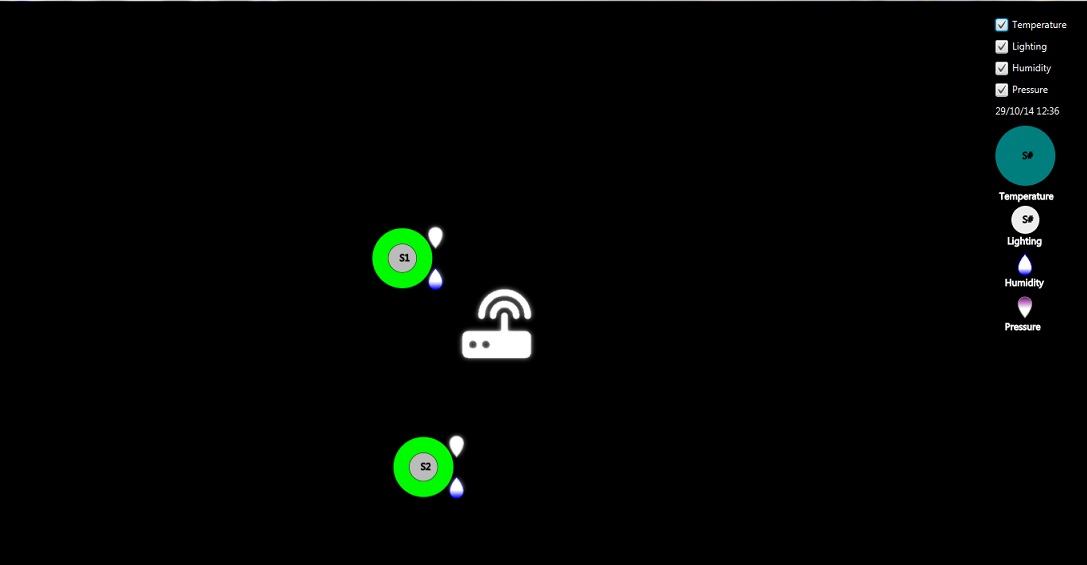
\includegraphics[width=\textwidth]{sprint_3/Sprint3Visualiser.png}
	\caption{Map View}
	\label{fig:map_view_3}
\end{figure}

\subsection{Customer Review}
The customer is happy about our progress, but he suggested that we implement some additional features if have enough time. The customer is interested in adding more gateways and sensors and hopes we could add as many as ten sensors and five gateways. Unfortunately we do not have time for a workload that is this big, this far in the project, so we might have to reduce the scope or maybe even drop the changes suggested all together.

The biggest problem we have is that we lack the hardware. The customer recommends that we use mock up data, but we felt that using mock up data in the final presentation is a step back, as we have done mock up data in sprint 1. While normally we would not have a problem with stepping back to progress forward, we feel that we might not have enough time to progress forward after the step back.

The customer also introduced us to a new function that the sensor has called link budget, which works like ping to calculate the position of the sensor from the central hub. During this meeting we did some basic tests and we found that the link budget increases drastically by walls or any kind of signal deterrent material, but did not increase as much by distance alone. A five metre walk changes the link budget by three or four units, while going behind a wall increased it by as many as twelve units. Going down a floor increased it by as many as fifteen units. The group concluded that under ideal conditions we can make positional triangulation work, but if there are any walls or link deterring materials, such as metal, the data will be completely different and quite unpredictable. The customer also mentioned the motion we have right now (we are using orbital movement to signify where the sensor might be) is wrong for the presentation, because the motion is not correct. 

To satisfy the customer needs, we will continue outside of our original plan and create a sprint 4. We may not have enough time to finish the implementation of sprint 4, but we will most likely be able to create something on a smaller scale. Still, with mock up data such an implementation will most likely only be there for the sake of presentation.

\subsection{Sprint Evaluation}
We have completed all of the goals of the sprint. We have fully integrated the system and we do not need any mock up data to run it. The system still retains the ability to connect to any database, with just a change in one line of code. By changing the IP or the address in the controller, we can connect to any database, containing real or mock up data.

We have also improved the look of the visualiser as well as added some new functionality. Besides adding a legend, representing what we are displaying on the screen, we have also added some subtle effects to make the visualiser look better. The response to these was positive. Finally, we have added a function that hides a sensor deemed “dead”. A sensor is deemed “dead” when it has not sent any data in the last hour. The visualiser then hides the sensor from display, but retain its previous data. Should the sensor “wake up” the visualiser will animate it once again without any disruption.

Finally, we have managed to complete all the tests successfully for this sprint. There are still some hardware difficulties and the sensors often do not register any data, which we can not fix, unfortunately. Still, besides the hardware failures we have managed to complete the overarching goal of the project, which is to visualize data gathered by the sensors. 

Our customer, however, wanted a much larger system without providing any additional hardware. To this end, we will attempt to create a final sprint with mock up data. We feel that this is a step backwards, since we used mock up data in earlier sprints, however, we will still attempt to complete as much as possible from the new request.

\end{document}
